\documentclass[11pt]{article}

\usepackage[english]{babel}
\usepackage[utf8]{inputenc}
\usepackage{graphicx}
\usepackage{framed}
\usepackage[normalem]{ulem}
\usepackage{amsmath}
\usepackage{amsthm}
\usepackage{amssymb}
\usepackage{amsfonts}
\usepackage{enumerate}
\usepackage[top=1 in,bottom=1in, left=1 in, right=1 in]{geometry}
\usepackage{listingsutf8}
\usepackage{color}
\usepackage{float}
\usepackage{graphicx}
\usepackage{subcaption}
\floatstyle{boxed} 
\restylefloat{figure}
\definecolor{mygreen}{rgb}{0,0.6,0}
\definecolor{mygray}{rgb}{0.5,0.5,0.5}
\definecolor{mymauve}{rgb}{0.58,0,0.82}

\lstset{ 
  backgroundcolor=\color{white},   % choose the background color; you must add \usepackage{color} or \usepackage{xcolor}; should come as last argument
  basicstyle=\footnotesize,        % the size of the fonts that are used for the code
  breakatwhitespace=false,         % sets if automatic breaks should only happen at whitespace
  breaklines=true,                 % sets automatic line breaking
  captionpos=b,                    % sets the caption-position to bottom
  commentstyle=\color{mygreen},    % comment style
  deletekeywords={...},            % if you want to delete keywords from the given language
  escapeinside={\%*}{*)},          % if you want to add LaTeX within your code
  extendedchars=true,              % lets you use non-ASCII characters; for 8-bits encodings only, does not work with UTF-8
  firstnumber=1000,                % start line enumeration with line 1000
  frame=single,	                   % adds a frame around the code
  keepspaces=true,                 % keeps spaces in text, useful for keeping indentation of code (possibly needs columns=flexible)
  keywordstyle=\color{blue},       % keyword style
  language=Octave,                 % the language of the code
  morekeywords={*,...},            % if you want to add more keywords to the set
  numbers=left,                    % where to put the line-numbers; possible values are (none, left, right)
  numbersep=5pt,                   % how far the line-numbers are from the code
  numberstyle=\tiny\color{mygray}, % the style that is used for the line-numbers
  rulecolor=\color{black},         % if not set, the frame-color may be changed on line-breaks within not-black text (e.g. comments (green here))
  showspaces=false,                % show spaces everywhere adding particular underscores; it overrides 'showstringspaces'
  showstringspaces=false,          % underline spaces within strings only
  showtabs=false,                  % show tabs within strings adding particular underscores
  stepnumber=2,                    % the step between two line-numbers. If it's 1, each line will be numbered
  stringstyle=\color{mymauve},     % string literal style
  tabsize=2,	                   % sets default tabsize to 2 spaces
  title=\lstname                   % show the filename of files included with \lstinputlisting; also try caption instead of title
}
\lstset{inputencoding=utf8/latin1}

\newcommand{\dt}{\partial_t}
\newcommand{\Tl}{\frac{T}{\lambda}}
\newcommand{\Dt}{\Delta t}
\newcommand{\Dx}{\Delta x}

\title{\textbf{Sur les schémas de l'équation ``KPP avec mémoire"}}
\author{Liam Toran}
\date{}
\begin{document}

\maketitle
\tableofcontents

\section{Schémas et Positivité}
On a le modèle suivant (``KPP avec mémoire"): 
\begin{equation} \left\{
                \begin{array}{ll}
                   \dt\mu = K\Delta\mu + C(\mu + \rho) -\mu\rho\\
                 \dt\rho=  F_0 \mu \\
                  \dt C = -b\rho C
                \end{array}
              \right.
\end{equation}
\subsection{Pour l'équation différentielle ordinaire}
Sans dépendance spatiale:
\begin{equation} \left\{
                \begin{array}{ll}
                   \dt\mu = C(\mu + \rho) -\mu\rho\\
                 \dt\rho=  F_0 \mu \\
                  \dt C = -b\rho C
                \end{array}
              \right.
\end{equation} 
\subsubsection{Schéma semi-implicite I pour l'EDO}
Soit le schéma semi-implicite I pour l'EDO:
\begin{equation} \boxed{\left\{
                \begin{array}{ll}
                   \mu^{n+1} = \mu^{n}+  \Dt( C^{n}(\mu^{n+1} + \rho^{n+1}) -\mu^{n+1}\rho^{n})\\
                \rho^{n+1}=  \rho^{n}+ \Dt (F_0 \mu^{n+1}) \\
                 C^{n+1} =C^{n}- \Dt(b\rho^{n+1}C^{n+1})
                \end{array}
              \right.}
\end{equation}
Ce schéma donne:
\begin{equation*} \left\{
                \begin{array}{ll}
                   \mu^{n+1}(1-\Dt(C^{n}(1+\Dt F_0)) + \rho^{n}) = \mu^{n}+  \Dt C^{n}\rho^{n} \\
                \rho^{n+1}=  \rho^{n}+ \Dt (F_0 \mu^{n+1}) \\
                 C^{n+1} =C^{n}\frac{1}{1+ \Dt b\rho^{n+1}}
                \end{array}
              \right.
\end{equation*}
Pour conserver la positivité il suffit que le terme $(1-\Dt(C^{n}(1+\Dt F_0)) + \rho^{n}) $ reste positif:\\
Par exemple: 
\begin{equation}
	\boxed{C^0< \frac{1}{\Dt(1+F_0\Dt)}}
\end{equation}

\subsubsection{Schéma semi-implicite II pour l'EDO}
Soit le schéma semi-implicite II pour l'EDO:
\begin{equation} \boxed{\left\{
                \begin{array}{ll}
                   \mu^{n+1} = \mu^{n}+  \Dt( C^{n}(\mu^{n+1} + \rho^{n+1}) -\mu^{n}\rho^{n})\\
                \rho^{n+1}=  \rho^{n}+ \Dt (F_0 \mu^{n+1}) \\
                 C^{n+1} =C^{n}- \Dt(b\rho^{n+1}C^{n+1})
                \end{array}
              \right.}
\end{equation}
Ce schéma donne:
\begin{equation*} \left\{
                \begin{array}{ll}
                   \mu^{n+1}(1-\Dt(C^{n}(1+\Dt F_0))) = \mu^{n}+  \Dt \rho^{n}(C^{n}-\mu^{n}) \\
                \rho^{n+1}=  \rho^{n}+ \Dt (F_0 \mu^{n+1}) \\
                 C^{n+1} =C^{n}\frac{1}{1+ \Dt b\rho^{n+1}}
                \end{array}
              \right.
\end{equation*}
Pour conserver la positivité il suffit que les terme $(1-\Dt(C^{n}(1+\Dt F_0)))$ et $\mu^{n}+  \Dt \rho^{n}(C^{n}-\mu^{n})$ restent positif:\\
Par exemple: 
\begin{equation}
	\boxed{C^0< \frac{1}{\Dt(1+F_0\Dt)}}
\end{equation}
et 
\begin{equation}
	\boxed{\rho^n< \frac{1}{\Dt}}
\end{equation}
On obtient une condition de plus que le schéma semi-implicite I.
\subsection{Pour l'équation aux dérivées partielles}
\subsubsection{Schéma semi-implicite I pour l'EDP}
Soit le schéma semi-implicite I pour l'EDP:
\begin{equation} \boxed{\left\{
                \begin{array}{ll}
                   \mu^{n+1}_i = \mu^{n}_i+ K\Dt \frac{\mu^{n+1}_{i+1}-2\mu^{n+1}_i+\mu^{n+1}_{i-1}}{\Dx ^2} + \Dt( C^{n}_i(\mu^{n+1}_i + \rho^{n+1}_i) -\mu^{n+1}_i\rho^{n}_i)\\
                \rho^{n+1}_i=  \rho^{n}_i+ \Dt (F_0 \mu^{n+1}_i) \\
                 C^{n+1}_i =C^{n}_i- \Dt(b\rho^{n+1}_iC^{n+1}_i)
                \end{array}
              \right.}
\end{equation}
Ce schéma donne:
\begin{equation*} \left\{
                \begin{array}{ll}
                   (1+\frac{K\Dt}{\Dx^2}A-\Dt(C^{n}(1+\Dt F_0)) + \rho^{n})\mu^{n+1} = \mu^{n}+  \Dt C^{n}\rho^{n} \\
                \rho^{n+1}=  \rho^{n}+ \Dt (F_0 \mu^{n+1}) \\
                 C^{n+1} = C^{n}\frac{1}{1+ \Dt b\rho^{n+1}}
                \end{array}
              \right.
\end{equation*}
où $A$ est la matrice de $-\Delta$
:\begin{equation}  \label{myeq}A= \left[ \begin{matrix}2 & -1 & & 0\\-1 & \ddots & \ddots &  \\& \ddots & \ddots &  -1 \\0 &  & -1 & 2  \end{matrix}  \right]\end{equation}
$A$ étant symétrique définie positive, afin de préserver la positivité, on obtient la même condition (suffisante) que pour l'EDO:
\begin{equation}
	\boxed{C^0< \frac{1}{\Dt(1+F_0\Dt)}}
\end{equation}
\newpage
\section{Résolution numérique}
\subsection{Résolution de l'EDO}
\subsubsection{Code de résolution de l'EDO}
\lstinputlisting[language=Python]{edo.py}
\subsubsection{Résultat de la simulation de l'EDO}
\begin{figure}[hbt!]
\centering
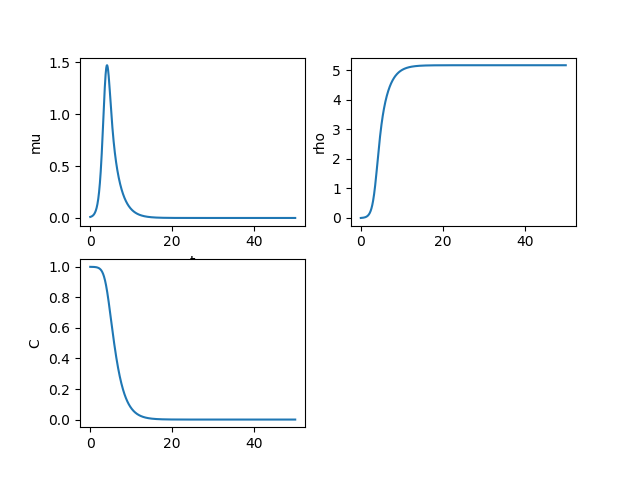
\includegraphics[width=.9\textwidth]{Images/edo_euler_implicite.png}
\caption{Résolution du schéma implicite pour l'EDO}
\end{figure}

\newpage
\subsection{Résolution de l'EDP en 1D}
\subsubsection{Code de la résolution de l'EDP en 1D}
\lstinputlisting[language=Python]{edp_1d.py}
\newpage
\subsubsection{Résultat de la simulation de l'EDP en 1D}
\begin{figure}[hbt!]
\centering
\begin{subfigure}[b]{0.45\textwidth}
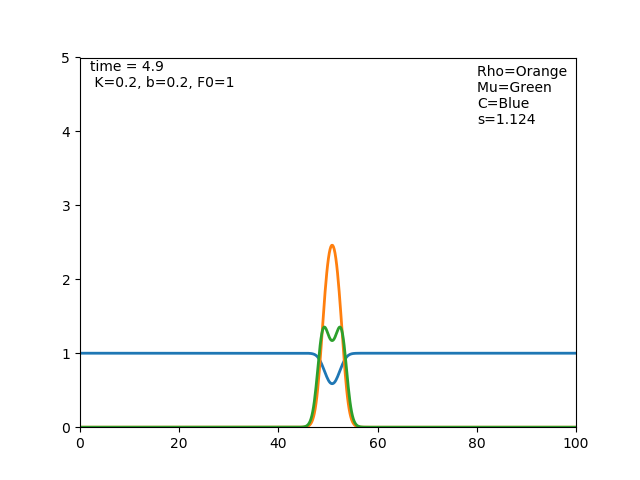
\includegraphics[width=\textwidth]{Images/edp_1d_0.png}
\end{subfigure}
\begin{subfigure}[b]{0.45\textwidth}
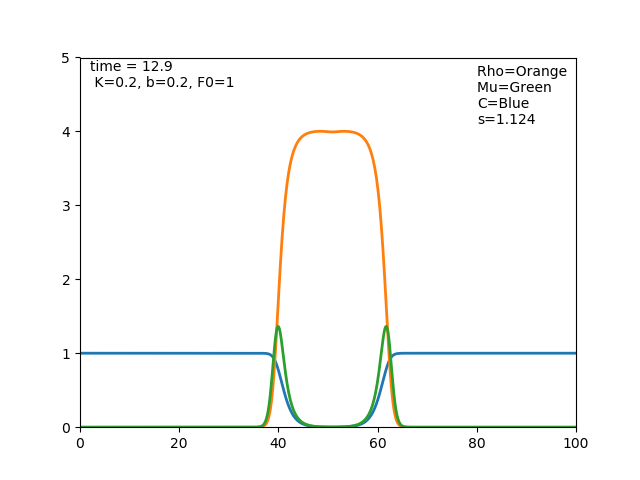
\includegraphics[width=\textwidth]{Images/edp_1d_1.png}
\end{subfigure}
\begin{subfigure}[b]{0.45\textwidth}
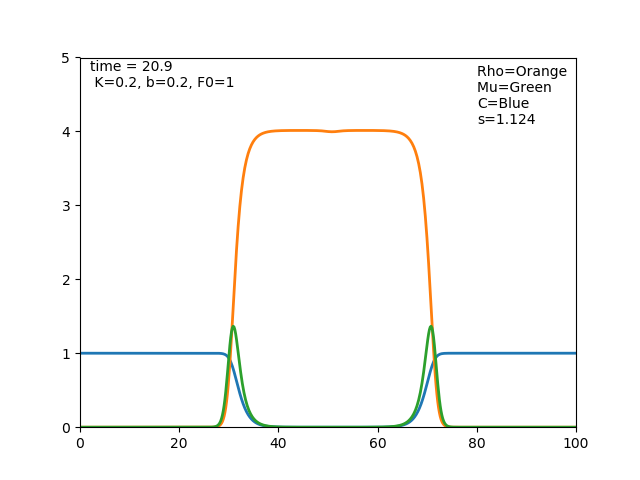
\includegraphics[width=\textwidth]{Images/edp_1d_2.png}
\end{subfigure}
\begin{subfigure}[b]{0.45\textwidth}
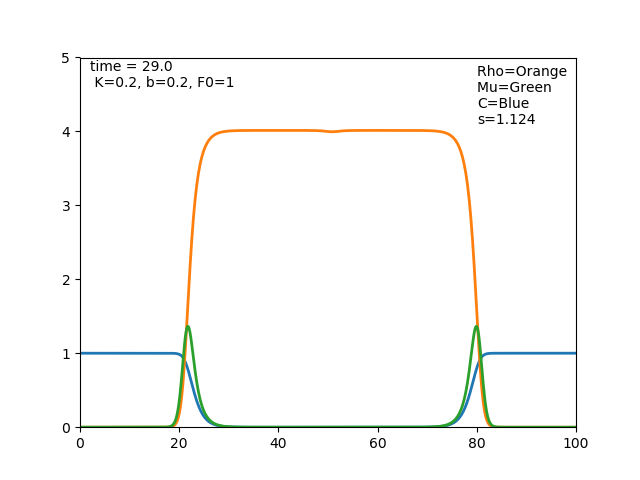
\includegraphics[width=\textwidth]{Images/edp_1d_3.png}
\end{subfigure}
\caption{Résolution du schéma semi implicite I pour l'EDP en 1D}
\end{figure}
\end{document}